% natbib guide (https://gking.harvard.edu/files/natnotes2.pdf)
% \citet     #textual citations, print the abbreviated author list
% \citet*    #textual citations, print the full author list
% \citep     #parenthetical citations, print the abbreviated author list
% \citep*    #parenthetical citations, print the full author list
% \citealt    #the same as \citet but without any parentheses.
% \citealp    #the same as \citep but without any parentheses. 
% \citeauthor{ale91}         #Alex et al.
% \citeauthor*{ale91}        #Alex, Mathew, and Ravi
% \citeyear{ale91}           #1991 
% \citeyearpar{ale91}        #(1991)

\documentclass[english, xcolor=dvipsnames, aspectratio=169]{beamer}

% Text encoding
\usepackage[english]{babel}

% Justify text (package and function)
% \apptocmd{command}{code}{success}{failure}
\usepackage{ragged2e}
\apptocmd{\frame}{}{\justifying}{} 
% Justify text in \item
\newcommand{\itemj}{\item \justifying}

% If...else package
\usepackage{ifthen}

% Package to set transparent background image
\usepackage{tikz}

% Include image package
\usepackage{graphicx}
% Set default path for images
\graphicspath{ {./imgs/} }
% Set figure number when included
\setbeamertemplate{caption}[numbered]

% Bibliography packages
\usepackage[sort, round]{natbib}
\bibliographystyle{plainnat}

% Define colors variables
\definecolor{red}{rgb}{0.631, 0.094, 0.094} % primary color
\definecolor{grey}{rgb}{0.3686, 0.5255, 0.6235} % secondary color

% Set theme palette colors
\setbeamercolor{palette primary}{bg=blue,fg=white}
\setbeamercolor{palette secondary}{bg=blue,fg=white}
\setbeamercolor{palette tertiary}{bg=blue,fg=white}
\setbeamercolor{palette quaternary}{bg=blue,fg=white}
% strucure means itemize, enumerate, etc
\setbeamercolor{structure}{fg=blue} 

% Set bibliography colors
\setbeamercolor{bibliography item}{fg=blue}
\setbeamercolor{bibliography entry author}{fg=black}
\setbeamercolor{bibliography entry title}{fg=black}
\setbeamercolor{bibliography entry location}{fg=black}
\setbeamercolor{bibliography entry note}{fg=black}
% Replaces book icon in bibliography with enumeration
\setbeamertemplate{bibliography item}{[\theenumiv]}

% Table of contents style
% \setbeamertemplate{section in toc}[sections numbered]
% \setbeamertemplate{subsection in toc}[subsections numbered]
\setbeamertemplate{section in toc}[circle]
\setbeamertemplate{subsection in toc}[ball unnumbered]

% Header with navigation bar
\setbeamertemplate{headline}
{
    \leavevmode
    \hbox{
    \begin{beamercolorbox}[wd=\paperwidth,ht=2.5ex,dp=1.125ex]{palette quaternary}
    \insertsectionnavigationhorizontal{\paperwidth}{}{\hskip0pt plus1filll}
    \end{beamercolorbox} 
    }
}
% Footer with custom caption
\setbeamertemplate{footline}
{
    \leavevmode
    \hbox{
    \begin{beamercolorbox}[wd=.33\paperwidth,ht=2.6ex,dp=1ex,center]{palette quaternary}
    \usebeamerfont{author in head/foot}\insertshortauthor\hspace*{1ex}
    \end{beamercolorbox}
    \begin{beamercolorbox}[wd=.33\paperwidth,ht=2.6ex,dp=1ex,center]{palette quaternary}
    \usebeamerfont{institute in head/foot}\insertshortinstitute
    \end{beamercolorbox}
    \begin{beamercolorbox}[wd=.33\paperwidth,ht=2.6ex,dp=1ex,center]{palette quaternary}
    \insertframenumber{} / \inserttotalframenumber
    \end{beamercolorbox}}
    \vskip0pt
}

% Global Background must be put in preamble
\usebackgroundtemplate
{
    \tikz\node[opacity=0.3]{
\includegraphics[height=\paperheight, width=\paperwidth]{background.png}};
}

% One line command to print table of contents - two parameters for modes
\newcommand{\customToC}[2]
{
    \begin{frame}{Overview}
    \tableofcontents[#1,#2]
    \end{frame}
}

% Command to plot centered figure
% Parameters: #1=image name, #2=caption 
\newcommand{\includefigure}[2]
{
    \begin{figure}[h]
    \caption{#2}
    \centering
    \includegraphics[width=0.5\textwidth]{#1}
    \end{figure}
}

% Command to set section name as variable (\renewcommand to update)
\newcommand{\sectiontitle}{}
% Command to set subsection name as variable (\renewcommand to update)
\newcommand{\subsectiontitle}{}


% Title page
\title{Title}
\subtitle{Subtitle}
\author{Author}
\institute{Università degli studi di Siena}
% Date
\day=01\relax
\month=01\relax
\year=2022\relax

\begin{document}

\frame{\titlepage}

% Complete table of contents (ToC)
% \customToC{hideallsubsections}{}
\customToC{}{}

% Section name and highlighted ToC
\renewcommand{\sectiontitle}{Section}
\section{\sectiontitle}
\customToC{currentsection,hideothersubsections}{}

\begin{frame}{\sectiontitle}
    This is some text in the first frame. This is some text in the first frame. This is some text in the first frame.
\end{frame}

% Section name and highlighted ToC
\renewcommand{\subsectiontitle}{Subsection}
\subsection{\subsectiontitle}
\begin{frame}{\subsectiontitle}
    \begin{itemize}
        \itemj Justified text item with reference \citet{goodfellow2014generative} 
        \item This is some unjustified text in the frame. This is some unjustified text in the frame. This is some unjustified text in the frame. This is some unjustified text in the frame. This is some unjustified text in the frame.
    \end{itemize}
    
    % Include figure with caption
    % \includefigure{gan_architecture.png}{Figure caption here}
        % Include figure with caption
    \begin{figure}
    \centering
        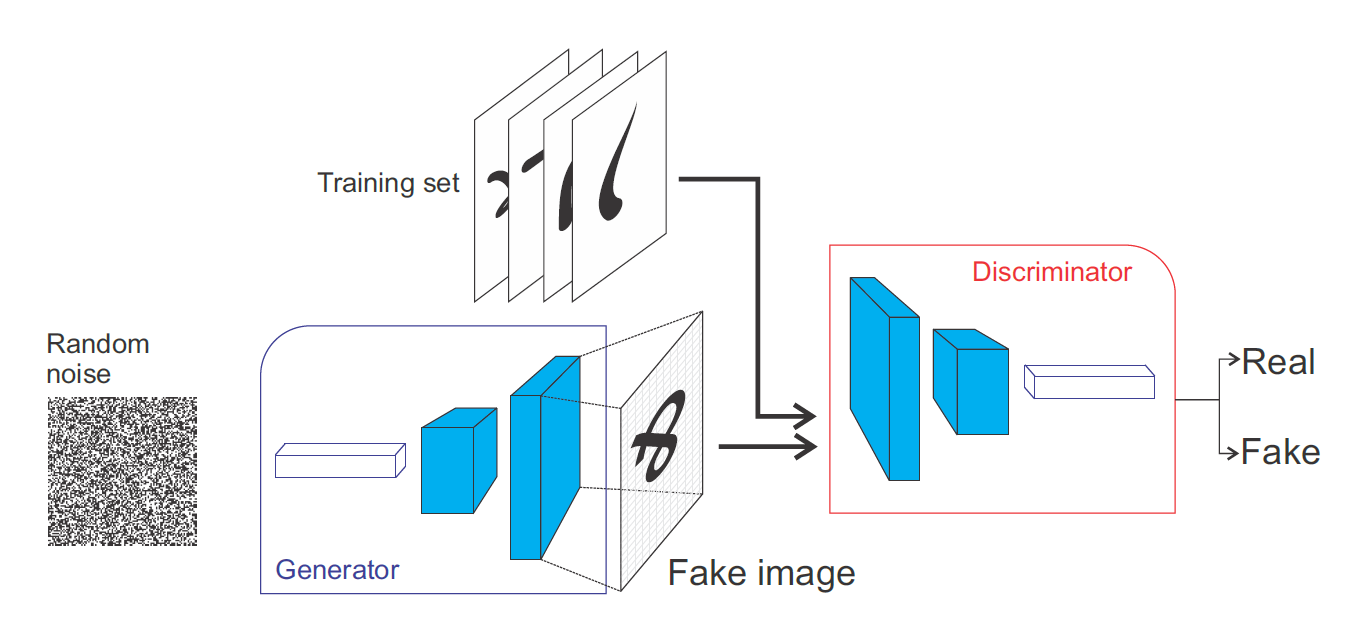
\includegraphics[width=.5\textwidth]{gan_architecture.png}
        \caption{GAN structure}
        \label{fig:gan_structure}
    \end{figure}
\end{frame}

% Section name and highlighted ToC
\renewcommand{\sectiontitle}{Another section}
\section{\sectiontitle}
\customToC{currentsection,hideothersubsections}{}

\begin{frame}{\sectiontitle}
    This is some text in the first frame. This is some text in the first frame. This is some text in the first frame.
\end{frame}

% Section name and highlighted ToC
\renewcommand{\subsectiontitle}{Subsection with math}
\subsection{\subsectiontitle}
% \customToC{currentsection,hideothersubsections}{}

\begin{frame}{\subsectiontitle}
    This is some text in the first frame. This is some text in the first frame. This is some text in the first frame.
    \begin{itemize}
    \itemj This is some text in the first frame. This is some text in the first frame. This is some text in the first frame.
    \itemj Example formula: $$d^2 = ||\mu_1 – \mu_2||^2 + Tr(C_1 + C_2 – 2\sqrt{C_1*C_2})$$ 
    \end{itemize}
\end{frame}

\renewcommand{\sectiontitle}{Section without frame}
\section{\sectiontitle}
\customToC{currentsection,hideothersubsections}{}

% Section name and highlighted ToC
\renewcommand{\subsectiontitle}{Subsection with table}
\subsection{\subsectiontitle}

\begin{frame}{\subsectiontitle}
\begin{table}[ht]
\caption{default}
\begin{center}
% \rowcolors{1}{}{red}
    \begin{tabular}{| c | c | c | c | c |}
    \hline
    \textbf{Dataset} & \textbf{No. Classes} & \textbf{Image Size} & \textbf{No.Images $S_t$} & \textbf{No.Images $S_v$} \\
    \hline
    MNIST & 10 & 28×28 & 60k & 10k \\
    \hline
    CIFAR10 & 10 & 32×32 & 50k & 10k \\
    \hline
    CIFAR100 & 100 & 32×32 & 50k & 10k \\
    \hline
    ImageNet1k & 1000 & 64×64/128×128 & 1.3M & 50k \\
    \hline
\end{tabular}
\end{center}
\end{table}
\end{frame}

% Section name and highlighted ToC
\renewcommand{\subsectiontitle}{Subsection with minipages}
\subsection{\subsectiontitle}
% \customToC{currentsection,hideothersubsections}{}

% Slide with four figures
\begin{frame}{\subsectiontitle}
    \begin{figure}[ht]
        \begin{minipage}[b]{0.45\linewidth}
            \centering
            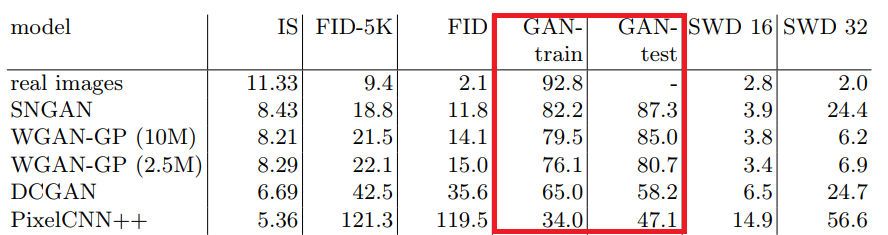
\includegraphics[width=\textwidth]{cifar10.png}
            \caption{Results on CIFAR10}
            \label{fig:cifar10}
        \end{minipage}
        \hspace{0.5cm}
        \begin{minipage}[b]{0.45\linewidth}
            \centering
            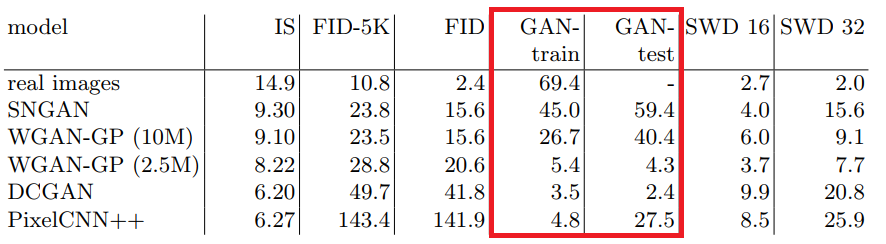
\includegraphics[width=\textwidth]{cifar100.png}
            \caption{Results on CIFAR100}
            \label{fig:cifar100}
        \end{minipage}
        \begin{minipage}[b]{0.45\linewidth}
            \centering
            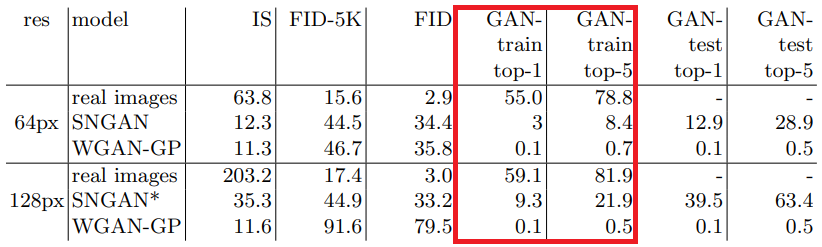
\includegraphics[width=\textwidth]{imagenet1k.png}
            \caption{Results on ImageNet 1k}
            \label{fig:imagenet1k}
        \end{minipage}
    \end{figure}
\end{frame}

% Import bibliography from file sample.bib
\begin{frame}[t, allowframebreaks]
\frametitle{References}
\bibliography{sample}
\end{frame}

\end{document}